\documentclass[journal]{new-aiaa}
%\documentclass[conf]{new-aiaa} for conference papers
\usepackage[utf8]{inputenc}

\usepackage{graphicx}
\usepackage{amsmath}
\usepackage[version=4]{mhchem}
\usepackage{siunitx}
\usepackage{longtable,tabularx}
\setlength\LTleft{0pt} 

\title{Preparation of Papers for AIAA Technical Journals}

\author{First A. Author\footnote{Insert Job Title, Department Name, Address/Mail Stop, and AIAA Member Grade (if any) for first author.} and Second B. Author Jr.\footnote{Insert Job Title, Department Name, Address/Mail Stop, and AIAA Member Grade (if any) for second author.}}
\affil{Business or Academic Affiliation 1, City, State, Zip Code}
\author{Third C. Author\footnote{Insert Job Title, Department Name, Address/Mail Stop, and AIAA Member Grade (if any) for third author.}}
\affil{Business or Academic Affiliation 2, City, Province, Zip Code, Country}
\author{Fourth D. Author\footnote{Insert Job Title, Department Name, Address/Mail Stop, and AIAA Member Grade (if any) for fourth author (etc.).}}
\affil{Business or Academic Affiliation 2, City, State, Zip Code}

\begin{document}

\maketitle

\begin{abstract}
These instructions give you guidelines for preparing papers for AIAA Technical Journals using \LaTeX{}. If you previously prepared an AIAA Conference Paper using the Papers Template, you may submit using the Papers Template so long as the text is double-spaced.  Carefully follow the journal paper submission process in Sec.~II of this document. Keep in mind that the electronic file you submit will be formatted further at AIAA. This first paragraph is formatted in the abstract style. Abstracts are required for regular, full-length papers and express articles. Be sure to define all symbols used in the abstract, and do not cite references in this section. The footnote on the first page should list the Job Title and AIAA Member Grade (if applicable) for each author.
\end{abstract}

\section*{Nomenclature}

\noindent(Nomenclature entries should have the units identified)

{\renewcommand\arraystretch{1.0}
\noindent\begin{longtable*}{@{}l @{\quad=\quad} l@{}}
$A$  & amplitude of oscillation \\
$a$ &    cylinder diameter \\
$C_p$& pressure coefficient \\
$Cx$ & force coefficient in the \textit{x} direction \\
$Cy$ & force coefficient in the \textit{y} direction \\
c   & chord \\
d$t$ & time step \\
$Fx$ & $X$ component of the resultant pressure force acting on the vehicle \\
$Fy$ & $Y$ component of the resultant pressure force acting on the vehicle \\
$f, g$   & generic functions \\
$h$  & height \\
$i$  & time index during navigation \\
$j$  & waypoint index \\
$K$  & trailing-edge (TE) nondimensional angular deflection rate\\
$\Theta$ & boundary-layer momentum thickness\\
$\rho$ & density\\
\multicolumn{2}{@{}l}{Subscripts}\\
cg & center of gravity\\
$G$ & generator body\\
iso	& waypoint index
\end{longtable*}}




\section{Introduction}
\lettrine{T}{his} document is a \LaTeX{} template for preparation of papers for AIAA Technical Journals. If you are reading a hard-copy or .pdf version of this document, download the electronic file, new-aiaa.cls, and use it to prepare your manuscript.

Authors using \url{https://www.overleaf.com} may simply open the AIAA template from the Overleaf gallery to work online; no local installation of any files is required. Authors using a local \LaTeX{} installation will need to open the template in Overleaf and use the ``Download as zip'' option from the project menu to download a local copy of the template files. To create your formatted manuscript, type your own text over sections of the template, or cut and paste from another document and then use the available markup styles. Note that special formatting such as subscripts, superscripts, and italics may be lost when you copy your text into the template from a Word Processing program such as Microsoft Word. See Sec. IV for more detailed formatting guidelines.


\section{Procedure for Paper Submission}

All manuscripts are to be submitted online at \url{https://mc.manuscriptcentral.com/aiaa}. Select either “Log In” if you have an existing account or “Create an Account” if this is your first time submitting to one of AIAA’s journals. If it’s the latter, please follow the instructions ScholarOne provides. Once you have logged into ScholarOne, select “Author Center” then scroll down. Under “Author Resources”, select the star beside “Click here to submit a new manuscript”. The site will take you step-by-step through the submission process. Once you submit your manuscript, you will receive an email containing your manuscript ID number as well as a link to view the status of your manuscript. 

After entering all required submission data, you must use the “Upload Manuscript” feature of the Author Center to upload your submission. Remember that your document must be in single-column, double-spaced format (as this template) before you upload it. Please be sure that the name of the file you upload for processing is short and simple (i.e., “SmithJPP.pdf”) with no spaces, tildes, symbols, or other special characters. Authors are encouraged to upload .pdf files, which are less likely to have conversion errors on upload. Failure to meet these requirements could result in a processing error that would require you to re-upload your manuscript. Once you have uploaded your manuscript, please inspect the file for accuracy. This step is required to complete your submission. If you experience difficulties with the upload and/or conversion of your manuscript, please contact ScholarOne Manuscripts Support (\url{https://mchelp.manuscriptcentral.com/gethelpnow/} or +1-888-503-1050) for additional assistance. 

\emph{Attention Asian Authors: If you are uploading a .pdf file, please remove Asian fonts from your file, under File>Properties.}

\section{General Guidelines}

The following section outlines general (nonformatting) guidelines to follow. These guidelines are applicable to all authors and include information on the policies and practices relevant to the publication of your manuscript.

\subsection{Publication by AIAA}
Your manuscript cannot be published by AIAA if:
\begin{enumerate}
\item The work is classified or has not been cleared for public release.
\item The work contains copyright-infringing material.
\item The work has been published or is currently under consideration for publication or presentation elsewhere. (Exception: Papers presented at AIAA conferences may be submitted to AIAA journals for possible publication.)
\end{enumerate}

You will be asked to provide the publication or presentation history of your paper (or any similar paper) if it has \emph{ever} been submitted for publication or presentation previously to an AIAA journal or conference. Please include the following, if applicable: the full name of the publication or conference, the entire paper number, dates the conference took place, review history, final disposition of manuscript, etc.


\subsection{Copyright}

Before AIAA can publish any paper, the copyright information must be completed in ScholarOne. Failure to complete the form correctly could result in your paper not being published. You must select one copyright assignment statement (select A, B, C, or D) and once a statement is picked, changes cannot be made during the proofs stage. Read the copyright statements carefully. AIAA requires a copyright transfer from the author(s) to AIAA or a license to print your material; government authors can assert that the work is in the public domain. Because you will be completing this form online, you do not need to fill out a hard-copy form. Do not include a copyright statement anywhere on your paper. The correct statement will be included automatically at the time of processing. (If your paper was presented at an AIAA conference, then the copyright statement chosen for the journal article should be the same as for your conference paper.)

\subsection{Publication Charges and Color Artwork}

Publication charges are voluntary, and nonpayment has no influence on the review process of the time from acceptance to publication. Publication charge payments help defray production costs and keep journal subscription prices low. 

The article publication charge for Open Access is available in ScholarOne and on the AIAA website; the fee is the same regardless of article type. Payment will guarantee that the article is Open Access immediately upon publication. Payment for Open Access also includes the cost of color reproduction in the print journals, if the author supplies color figures.

Authors also may pay for color reproduction of their figures in the print journals, even if they do not pay for Open Access. The Color Charges for each article type vary and are available in ScholarOne and on the AIAA website.

Authors who submit color artwork but do not pay the Publication Charges will have their illustrations printed in black and white in print versions of the journals. Payment details and instructions will be provided to authors during production of the final article. 

\section{Instructions}

If you are using the AIAA Journals \LaTeX{} Template file to prepare your manuscript, you can simply type your own text over sections of this document, or cut and paste from another document and use the available markup styles. If you choose to cut and paste, select the text from your original document and choose Edit>Copy. (Do not select your title and author information, since the document spacing may be affected. It is a simple task to reenter your title and author information in the template.) Open the Journals Template. Place your cursor in the text area of the template and select Edit>Paste. Please note that special formatting (e.g., subscripts, superscripts, italics) may be lost when you copy your text into the template.

To apply the AIAA Journals formatting, use the standard \LaTeX{} commands for sections and subsection, etc; all the styles you will need to format your document are available as standard \LaTeX{} commands. The style will automatically adjust your fonts and line spacing. Repeat this process to apply formatting to all elements of your paper. \emph{Do not change the font sizes, line spacing, or margins. Do not manually hyphenate your document.} Use italics for emphasis; do not underline. 

Use the Print option under the File tab to view Page Layout and see the most accurate representation of how your final paper will appear. Once formatting is complete, be sure to double space all sections of your manuscript.


\subsection{Document Text}
The default font for the Template is Times New Roman, 10-point size. The first line of every paragraph should be indented, and all lines should be double-spaced. Default margins are 1 in. on all sides. In the electronic version of this template, all margins and other formatting are preset. There should be no additional (blank) lines between paragraphs.

\emph{NOTE:} If you are using the Template to format your manuscript, the required spacing and formatting will be applied automatically.


\subsection{Headings}
Format the title of your paper in bold, 18-point type, with capital and lower-case letters, and center it at the top of the page. The names of the authors, business or academic affiliation, city, and state/province follow on separate lines below the title. The names of authors with the same affiliation can be listed on the same line above their collective affiliation information. Author names are centered, and affiliations are centered and in italic type. The affiliation line for each author includes that author’s city, state, and zip/postal code (or city, province, zip/postal code and country, as appropriate). The first footnote (bottom of first page) contains the job title and department name, and AIAA member grade for each author. Author email addresses may be included also.

Major headings in the template (``sections'' in the \LaTeX{} template commands) are bold 11-point font and centered. Please omit section numbers before all headings unless you refer frequently to different sections. Use Roman numerals for major headings if they must be numbered.

Subheadings (``subsections'' in the \LaTeX{} template commands) are bold, flush left, and either unnumbered or identified with capital letters if necessary for cross-referencing sections within the paper. There must be at least 2 of all subheadings and sub-subheadings. If there is only a single subheading or sub-subheading, please italicize the title of the subheadings, followed by a period, and run it into the text paragraph. 

Sub-subheadings (``subsubsections'' in the \LaTeX{} template commands) are italic, flush left, and either unnumbered or numbered with Arabic numerals (1, 2, 3, etc.) if necessary for cross-referencing sections within the paper.


\subsection{Abstract}
An abstract appears at the beginning of Full-Length Papers, Regular Articles, and Express Articles. (Survey and Design Forum Papers, History of Key Technologies Papers, invited lectures, and Technical/Engineering Notes do not include abstracts.) The abstract is one paragraph (not an introduction) and complete in itself (no reference numbers). It should indicate subjects dealt with in the paper and state the objectives of the investigation. Newly observed facts and conclusions of the experiment or argument discussed in the paper must be stated in summary form; readers should not have to read the paper to understand the abstract. Format the abstract bold, indented 3 picas (1/2 in.) on each side, and separated from the rest of the document by two blank lines.


\subsection{Nomenclature}
Papers with many symbols may benefit from a nomenclature list that defines all symbols with units, inserted between the abstract and the introduction. If one is used, it must contain all the symbology used in the manuscript, and the definitions should not be repeated in the text. In all cases, identify the symbols used if they are not widely recognized in the profession. Define acronyms in the text, not in the nomenclature. 

\subsection{Biographies}
Survey Papers and some Full-Length Papers include author biographies. These biographies are one paragraph each and should use the abstract formatting style.

\subsection{Footnotes and References}
Footnotes, where they appear, should be placed above the 1'' margin at the bottom of the page. To insert footnotes into the template, use the Insert>Footnote feature from the main menu as necessary. Footnotes are formatted automatically in the template, but if another medium is used, should appear in superscript as symbols in the sequence, *, $\dag$, $\ddag$, \S, \P, **, $\dag\dag$, $\ddag\ddag$, \S\S, etc.

List and number all references at the end of the paper. Corresponding bracketed numbers are used to cite references in the text \cite{vatistas1986reverse}, including citations that are an integral part of the sentence (e.g., ``It is shown in \cite{dornheim1996planetary} that\ldots '') or follow a mathematical expression: ``$A^{2} + B = C$ (Ref.~\cite{terster1997nasa}).'' For multiple citations, separate reference numbers with commas \cite{peyret2012computational,oates1997aerothermodynamics}, or use a dash to show a range \cite{volpe1994techniques,thompsonspacecraft,chi1993fluid}. Reference citations in the text should be in numerical order.

In the reference list, give all authors' names; do not use ``et al.'' unless there are six authors or more. Papers that have not been published should be cited as ``unpublished''; papers that have been submitted or accepted for publication should be cited as ``submitted for publication.'' Private communications and personal website should appear as footnotes rather than in the reference list.

References should be cited according to the standard publication reference style (for examples, see the ``References'' section of this template). Never edit titles in references to conform to AIAA style of spellings, abbreviations, etc. Names and locations of publishers should be listed; month and year should be included for reports and papers. For papers published in translation journals, please give the English citation first, followed by the original foreign language citation.

\subsection{Figures and Tables}
Insert tables and figures within your document; they may be either scattered throughout the text or grouped all together at the end of the file. Do not insert your figures in text boxes. Figures should have no background, borders, or outlines. In the \LaTeX{} template, use the ``caption'' command to type caption text. Captions are bold with a single tab (no hyphen or other character) between the figure number and figure description. See the Table 1 example for table style and column alignment. If you wish to center tables that do not fill the width of the page, simply highlight and “grab” the entire table to move it into proper position.


\begin{table}[hbt!]
\caption{\label{tab:table1} Transitions selected for thermometry}
\centering
\begin{tabular}{lcccccc}
\hline
& Transition& & \multicolumn{2}{c}{}\\\cline{2-2}
Line& $\nu''$& & $J'' $& Frequency, cm$^{-1}$& $FJ$, cm$^{-1}$& $G\nu $, cm$^{-1}$\\\hline
a& 0& P$_{12}$& 2.5& 44069.416& 73.58& 948.66\\
b& 1& R$_{2}$& 2.5& 42229.348& 73.41& 2824.76\\
c& 2& R$_{21}$& 805& 40562.179& 71.37& 4672.68\\
d& 0& R$_{2}$& 23.5& 42516.527& 1045.85& 948.76\\
\hline
\end{tabular}
\end{table}


\begin{figure}[hbt!]
\centering
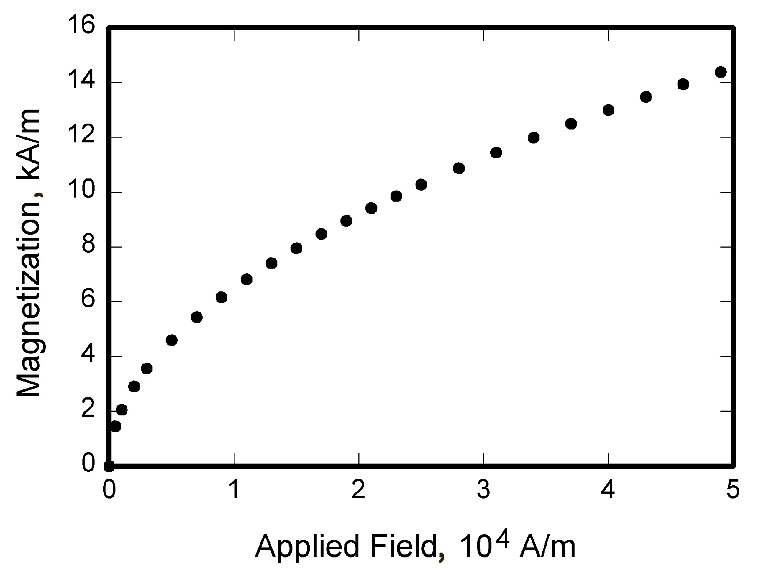
\includegraphics[width=.5\textwidth]{graph}
\caption{Magnetization as a function of applied fields.}
\end{figure}

Line drawings must be clear and sharp. Make sure that all lines and graph points are dark and distinct and that lettering is legible; 8- to 10-point type is suitable for artwork that is sized to fit the column width (3 ¼ in.). Keep the lettering size and style uniform both within each figure and throughout all of your illustrations. Place figure captions below each figure, and limit caption length to 20-25 words. If your figure has multiple parts, include the labels “a),” “b),” etc., below and to the left of each part, above the figure caption. Please verify that the figures and tables you mention in the text actually exist. When citing a figure in the text, use the abbreviation “Fig.” except at the beginning of a sentence. Do not abbreviate “Table.” Number each different type of illustration (i.e., figures and tables) sequentially with relation to other illustrations of the same type.

Figure labels must be legible after reduction to column width (preferably 8--10 points after reduction).

Note: If you wish to submit color figures (photographs or line art) for reproduction in the print format of a journal, publication charges must be paid. Black and white versions of color images must be supplied if the color fee is not paid. More than one color will translate to black when reproduced in gray scale, which leads to non-unique mapping of elements within the figure, so be sure to supply figures where legends progress monotonically and uniquely from light gray to dark gray.

All tables are numbered consecutively and must be cited in the text; give each table a definitive title. Be sure that you have a minimum of two columns (with headings) and two rows to constitute a proper table; otherwise reformat as a displayed list or incorporate the data into the text. Plan tables to fit the column width (3 ¼ in.) or the journal page width (7 in.). Position a double rule at the top and bottom of each table and single rule under the column headings; do not use shading, border lines, or vertical rules between table columns. Position each table in the text close to where it is cited


\subsection{Equations}
Equations are numbered consecutively, with equation numbers in parentheses flush right, as in Eq.~\eqref{sample:equation}. Insert a blank line on either side of the equation. To insert an equation into the \LaTeX{} document, use the \verb|\begin{equation}...\end{equation}| command environment.

A sample equation is included here, formatted using the preceding instructions:

\begin{equation}
\label{sample:equation}
\int^{r_2}_0 F(r,\varphi){\rm d}r\,{\rm d}\varphi = [\sigma r_2/(2\mu_0)]\int^{\infty}_0\exp(-\lambda|z_j-z_i|)\lambda^{-1}J_1 (\lambda r_2)J_0 (\lambda r_i\,\lambda {\rm d}\lambda)
\end{equation}

Be sure that symbols in your equation are defined in the Nomenclature or immediately following the equation. Also define abbreviations and acronyms the first time they are used in the main text. (Very common abbreviations such as AIAA and NASA, do not have to be defined.)

\subsection{General Grammar and Preferred Usage}
Use only one space after periods or colons. Hyphenate complex modifiers: ``zero-field-cooled magnetization.'' Insert a zero before decimal points: ``0.25,'' not ``.25.'' Use ``\si{\centi\meter\squared}'' not ``cc.'' 

A parenthetical statement at the end of a sentence is punctuated outside of the closing parenthesis (like this). (A parenthetical sentence is punctuated within parenthesis.) Use American, not English, spellings (e.g., “color,” not “colour”). The serial comma is preferred: “A, B, and C” instead of “A, B and C.”

Be aware of the different meanings of the homophones “affect” (usually a verb) and “effect” (usually a noun), “complement” and “compliment,” “discreet” and “discrete,” “principal” (e.g., “principal investigator”) and “principle” (e.g., “principle of measurement”). Do not confuse “imply” and “infer.”

\section{Conclusion}
Although a conclusion may review the main points of the paper, it must not replicate the abstract. A conclusion might elaborate on the importance of the work or suggest applications and extensions. Do not cite references in the conclusion. Note that the conclusion section is the last section of the paper to be numbered. The appendix (if present), funding information, other acknowledgments, and references are listed without numbers.

\section*{Appendix}

An Appendix, if needed, appears \textbf{before} research funding information and other acknowledgments.

\section*{Funding Sources}

Sponsorship information and acknowledgments of financial support should be included here. \textbf{Authors are responsible for accurately reporting funding data relevant to their research.} Please confirm that you have correctly entered \textbf{all sources} of funding and grant/award numbers \textbf{for all authors} in this section of your article. You will also be asked to select the appropriate funding organization from a drop-down menu in ScholarOne when you submit your manuscript. Be careful to choose the correct funder name, as organization names can be similar, and also be mindful to select sub-organizations within the registry hierarchy that are the actual funding sources, as appropriate, rather than choosing the name of the parent organization. Information provided in your manuscript must match the funding data entered in ScholarOne.

\section*{Acknowledgments}
An Acknowledgments section, if used, \textbf{immediately precedes} the References. Individuals other than the authors who contributed to the underlying research may be acknowledged in this section. The use of special facilities and other resources also may be acknowledged. 

\bibliography{sample}

\end{document}
